\chapter{\texttt{DigitClassifier} node}
	\label{chap:4_digitclassifier}
	\section{Description}
	\section{Functional architecture}
	\section{Neural Network processing}
		This JdeRobot component\footnote{\url{https://github.com/JdeRobot/dl-digitclassifier}} was originally designed by David Pascual \cite{dpascualhe} and Nuria Oyaga \cite{noyaga}, and it was used on this project to land on the concept of neural networks.\\
		
		Its design aims to \textit{classify handwritten numbers} with the use of a Convolutional Neural Network (\autoref{sec:1_cnn}), that classifies the incoming images from a video source.\\
		
		\begin{figure}[h]
			\centering
			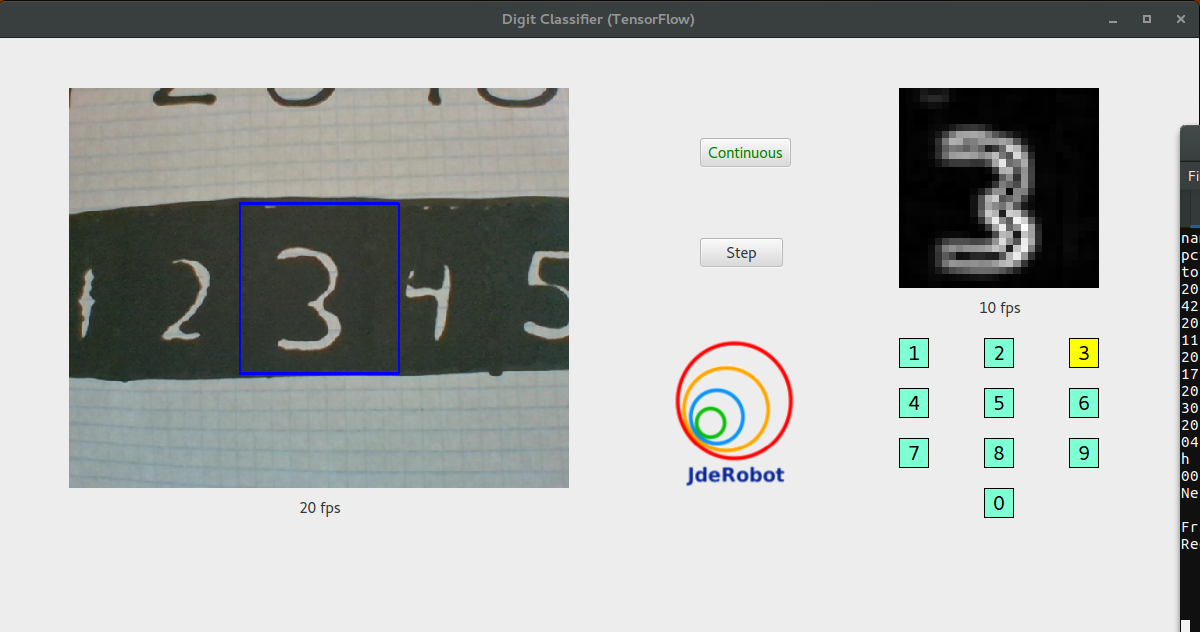
\includegraphics[width=4in]{images/digitclassifier}
			\caption{\texttt{DigitClassifier} on action.}
			\label{fig:4_digitclassifier}
		\end{figure}
			
			The previous implementations were written in Keras and Caffe (Python libraries to implement Neural Networks), so we made the same on TensorFlow (\autoref{sec:3_tensorflow}), to accomplish an initial domain of this Machine Learning framework.\\
			
			The implementation of this convolutional neural network consists on a concatenation of layers, following the scheme shown on \autoref{fig:3_digitclassifier_neural_structure}, which perform specific operations.
			
			\begin{figure}[h]
				\centering
				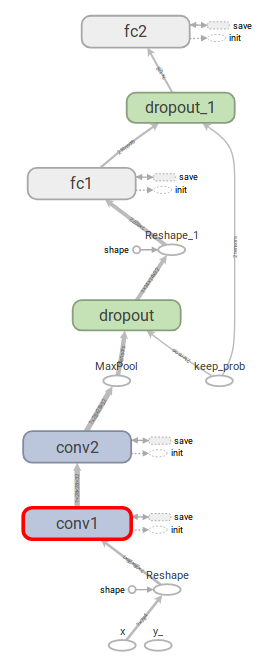
\includegraphics[width=2in]{images/digitclassifier_network_graph}
				\caption{Digit classifying neural structure.}
				\label{fig:3_digitclassifier_neural_structure}
				\end{figure}
				
				
				
				\begin{enumerate}
					\item \texttt{conv1}: first convolutional layer. As described in \autoref{sec:1_cnn}, it performs a 2D convolution between a $5px \times 5px$ square mask\/kernel (\texttt{W\_conv1}), and then adds a bias/intercept term (\texttt{b\_conv1}).\\
					\item \texttt{conv2}: second convolutional layer. It performs the same operation taking the output from the previous layer as an input, using a different weights mask and bias terms.\\
					
					Until now, what we have done is extracting patterns on each digit type (e.g. discovering typical circles on $0$ and $8$, which are always present on the same zone of the image).\\
					\item \texttt{pooling}: as the activation maps can be growing in size as we perform feed forward propagation, a \emph{pooling} operation is performed. It consists on sampling the input. Concretely, we retain the \textit{maximum} value for each 2 pixels, which is known as \textit{$2x2$ \texttt{max pooling}}
					
					\item \texttt{dropout}: this layer does not strictly perform any mathematical operations. It lets pass the TENSORS through it, but randomly switching off some neurons. This is parameterized by a user input, using a variable called \texttt{keep\_prob}. In our case, we set it to $0.5 (50\%)$ during the training process, to avoid overfitting by forcing the network to modify the neural paths randomly, as not every neuron is available on every moment. This is kind of similar to augmenting the dataset during the training process. The rest of the time (when the network is used to make inferences), this parameter is set to $1.0$, which means that no neurons are switched off at all.\\
					\item \texttt{fc1}: first fully connected layer. These layers, also known as \emph{dense} layers, are distinguised because every neuron is connected to every activation from the previous layer. So, this kind of layers are used for \textit{pattern association with labels}, due to the relationship they can infer between every input.\\
					\item \texttt{fc2}: the output layer. It connects all the outputs of the previous dense layer and groups the output in a 10-dimensional vector, which contains the probability of the digit to belong to each one of the possible classes.
					\end{enumerate}
					
					
					
					Once all this was achieved, we upgraded the code (from single ICE support to ROS+ICE via the \texttt{comm} library), and unified it (Keras + TensorFlow frameworks in a single component, under choice using the YML configuration file) on the official JdeRobot repository. From there it can be used right out of the box with the included model for both frameworks. In addition, you can train your own models using the provided datasets, or yours if you build another.
					


\chapter{\texttt{ObjectDetector} node}
\section{Description}
\section{Functional architecture}
\section{Neural Network processing}


\chapter{\texttt{FollowPerson} node}
\label{chap:followperson}
\section{Description}
\section{Functional architecture}
\section{Neural Network processing}
\section{Face detection and identification}
\section{Tracking algorithm}
\section{Physical response (\emph{PID} controller)}
\section{Experiments}
\subsection{Alternative approach: PTZ Camera}
\label{sec:follow_ptz}


\chapter{Conclusions}
	\section{Conclusions}
	\section{Future research lines}